\documentclass{scrartcl}
\usepackage{tabularx}
\usepackage{booktabs}
\usepackage{csquotes}
% Include Graphic-files:
\usepackage{graphicx}
\usepackage{caption}
\usepackage{subfig}
\usepackage{url}
%\usepackage{subfig}
\newsubfloat{figure}
\newcommand{\source}[1]{\vspace{-3pt} \caption*{ Source: {#1}} }

\begin{document}

\begin{figure}[!t]
\hskip 22pt
  \begin{minipage}[!t]{0.4\textwidth}
    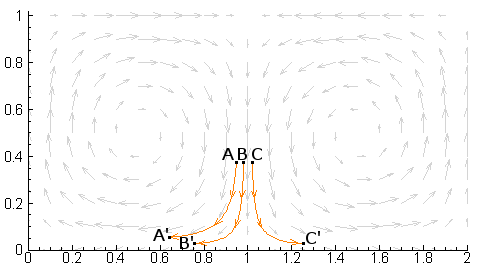
\includegraphics[width=\textwidth]{img/diverge.png}
	a)
   \label{diverge}
   \captionsetup{font={footnotesize,bf,it}}
  \end{minipage} \hskip 30pt
  %\raggedright
  \begin{minipage}[!t]{0.4\textwidth}
    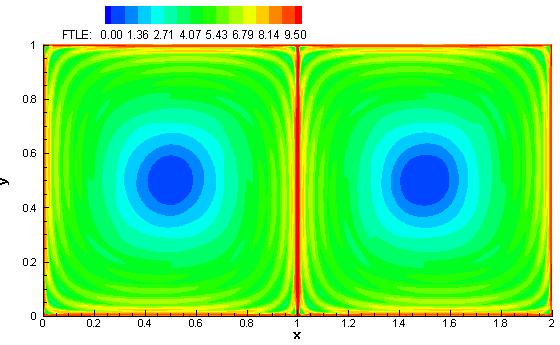
\includegraphics[width=\textwidth]{img/ftle_gyre.png}
	b)
    \captionsetup{font={footnotesize,bf,it}}
  \end{minipage}
  \caption{double gyre: a) diverging streamlines, b) FTLE field}
  \label{ftle_gyre}
  \caption*{source: \url{https://shaddenlab.berkeley.edu/uploads/LCS-tutorial/}}
\end{figure}
%%%%%%%%%%%%%%%%%%%%%%%%%%%%%%%%%%%%%%%%%%%%%%%%%%%%%%%%%%%%

% Alternative: put content in separate files
% Check the difference between including these files using \input{filename} and \include{filename} and see which one you like better
%\chapter{Einleitung}\label{intro}
%\input{introduction}
%
%\chapter{Voraussetzungen}\label{bg}
%\input{background}



\end{document}